\documentclass{article}
\usepackage[margin=1in]{geometry}
\usepackage{microtype}
\usepackage{flafter}
\usepackage{graphicx} % Required for inserting images
\usepackage{enumitem} % Required for itemize options in normative table
\usepackage{amssymb} % Required for \square symbol
\usepackage[super,sort&compress]{natbib}
\usepackage{url}  % handles special chars in URLs/DOIs in bibliography

\usepackage{color}
\definecolor{darkblue}{rgb}{0,0.08,0.35}
\definecolor{darkgreen}{rgb}{0,0.35,0.08}
\usepackage[backref=false,breaklinks,colorlinks,citecolor=darkblue,linkcolor=darkgreen,urlcolor=darkblue,hyperindex,plainpages=false,pdftex]{hyperref} % Hyper-references



% Scientific Data: max 110 chars, no colons or parentheses, capitalize only first word + proper nouns
\title{STAMPED principles for reproducible research objects}
\author{Austin Macdonald, Cody C. Baker, Isaac To, Yaroslav O. Halchenko}
\date{March 2026}

\begin{document}

\maketitle

\section{Abstract}

% TODO: compose later when other stuff filled out

\section{Introduction}

Data-driven research depends on specific versions of datasets, software, and computational environments, and a record of how they were used together to produce results.
We adopt the term \textbf{research object} to denote a collection of data, code, and metadata that together represent the research as a complete unit.
It is common for the components of a research object to be organized independently with code in one repository, data on a shared drive, environment setup in a wiki page, provenance in a lab notebook or nowhere at all.
This separation undermines rigor, reproducibility, reusability, and efficiency.
Even when its components are gathered in one place, a research object is often tightly coupled to specific environments, opaque to outside collaborators, and difficult to reuse or redistribute.

The FAIR principles\cite{wilkinson_fair_2016} and FAIR4RS guidelines\cite{barker_introducing_2022} provide structured guidance for making digital objects "Findable, Accessible, Interoperable, and Reusable".
The Workflow Community Initiative (WCI-FW)\cite{wilkinson_applying_2025} mapped these principles onto computational workflows but explicitly chose not to define new ones, instead treating workflows as hybrid data \& software objects.
STAMPED addresses a complementary question: how a research object should be organized and managed so it can actually be re-executed, extended, and redistributed.
Both the FAIR and STAMPED frameworks cover overlapping concerns.
For example, persistent identifiers serve both Findability and Tracking, but accent different aspects: FAIR emphasizes discovery and interoperability across repositories, while STAMPED emphasizes improving the operational maturity of scientific workflows in day-to-day research practice.

Many researchers already employ practices that address these operational properties, such as version control, containerized environments, structured project directories, and documented analysis steps. % TODO: It is unclear what the operational properties are at this point, so it can be confusing to the user.
Yet the community lacks a shared vocabulary for referring to these ideas, evaluating how thoroughly they are applied, and communicating that evaluation to collaborators and reviewers.
Here we provide that vocabulary by introducing seven principles which articulate how Self-contained, Tracked, Actionable, Modular, Portable, Ephemeral, and Distributable (STAMPED) a research object is, thus describing its operational maturity.
These originate from both the YODA Principles\cite{hanke_yoda_2018}, as well as VAMP\cite{hanke_what_2023}.
Rather than a compliance threshold, each STAMPED principle is a spectrum from a practical minimum---often what researchers are already doing---to an aspirational ideal.
A researcher who stores everything under one project directory, version-controls analysis scripts, and documents how to run them is already meeting the practical minimum for Self-containment, Tracking, and Actionability.
As complexity grows, such as for multi-institutional collaborations with heterogeneous workflows spanning platforms enforcing long-term reproducibility, these same principles guide researchers toward more rigorous practices without requiring wholesale adoption of new tools.
STAMPED provides a vocabulary for describing and a framework for evaluating and incrementally improving the operational properties of research objects toward enhanced rigor, reproducibility, reusability, and efficiency.

\begin{figure}[htbp]
\centering
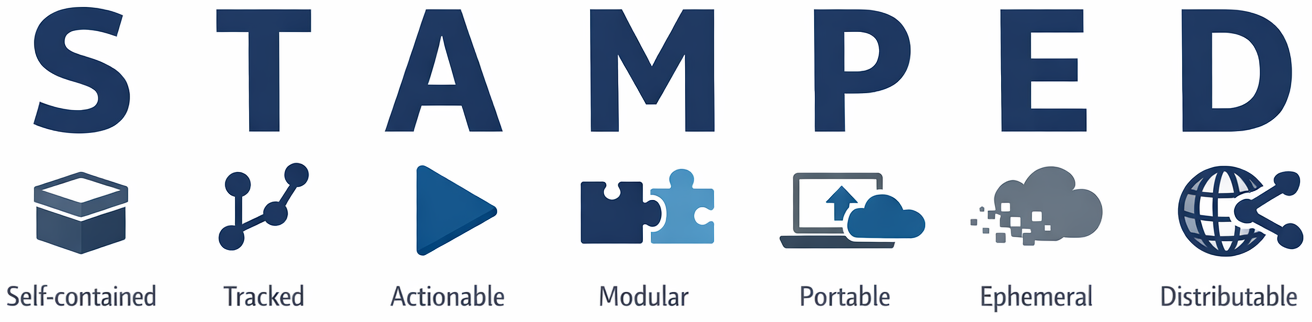
\includegraphics[width=\textwidth]{figures/fig1.png}  % TODO: vectorize and humanize
\caption{Illustration of the STAMPED principles.}
\label{fig:stamped}
\end{figure}



\section{Comments}

\begin{table}[htbp]
\centering
\caption{The STAMPED Principles where each one addresses a distinct property of research object organization that contributes to reproducibility. Together, they provide a framework for evaluating and improving the reproducibility of computational research.}
\label{tab:stamped}
\begin{tabular}{c l p{0.65\textwidth}}
\hline
\textbf{Letter} & \textbf{Principle} & \textbf{Description} \\
\hline
S & Self-containment & A research object is a complete retrieval unit; it can be obtained and understood in its intended scope without needing to reference external resources. \\
T & Tracking & The state and provenance of all components is recorded. \\
A & Actionability & Research object contains machine-actionable information to carry out procedures to obtain or reproduce content. \\
M & Modularity & All modules are independent and composable. \\
P & Portability & Research object could be moved to different environments while retaining its STAMPED properties. \\
E & Ephemerality & Procedural execution is performed within a throwaway environment. \\
D & Distributability & All modules and procedures are shareable externally in a persistent state. \\
\hline
\end{tabular}
\end{table}

The items containing keywords "MUST", "SHALL", "SHOULD", and "MAY" are to be interpreted as described in RFC 2119\cite{bradner_key_1997}.



\subsection{Self-containment}

\begin{itemize}
    \item \textbf{S.1}: All modules and components essential to replicate computational execution MUST be reachable within a single top-level research object.
\end{itemize}

Reproducibility fails when a research object depends on resources that are not part of it; an undocumented library, a dataset referenced by a broken URL, a script that assumes tools are installed on the host system.
We call this the ``don't look up'' rule: a research object must never rely on implicit external state.
Instead, it must be a complete retrieval unit, where all modules and components essential to reproduce its results are contained within a single top-level boundary (S.1, Table~1).

Components may be included literally (e.g., files committed directly) or by reference (e.g., as subdatasets, registered data URLs).
Both approaches satisfy self-containment, provided the references are explicit and part of the research object.
At a minimum, everything needed is gathered under one root and any external dependency is explicitly documented.
This ensures that nothing is implicitly assumed about the host system, a concern further addressed by Portability.
At the ideal end, every reference is precise enough that retrieval is unambiguous; how to achieve that precision is the concern of Tracking (T) and Distributability (D).

Self-containment is the foundation upon which the remaining STAMPED principles are built.
Tracking, Modularity, Portability, and Distributability each address a different aspect of how that boundary is organized, versioned, and shared---but none are meaningful without first establishing what is inside it.



\subsection{Tracking}

\begin{itemize}
    \item \textbf{T.1}: Persistent content identification MUST be recorded for all components.
    \item \textbf{T.2}: All components SHOULD be tracked using the same content-addressed version control system.
    \item \textbf{T.3}: Provenance of all modifications MUST be recorded.
    \item \textbf{T.4}: Code-driven provenance SHOULD be recorded programmatically and MUST include the versions of
    all components involved.
\end{itemize}

Research data and code change constantly during a project, and each change compounds the difficulty of reconstructing any previous state: which version of a dataset was used for a particular analysis, what parameters were set, what code produced a given figure.
Tracking addresses two concerns: 1) the identity of each component and its exact state at a point in time, and 2) \textbf{provenance}, the recorded history of what actions by which identities produced or modified it.
These are often managed separately, which makes prior work harder to validate.

The spectrum of Tracking begins with content-addressed version control.
Rather than relying on semantic version labels, content-addressed systems identify each state by a checksum of its contents.
This distinction matters: two datasets labeled ``version 1.0'' by different labs are ambiguous; two datasets with identical content hashes are provably identical.
Version control commits also capture basic provenance: who made the change, when, and a description of why.
This unifies identity and provenance in a single system and also provides a safety net since any change can be reverted and any prior state restored, making it easier to modify and experiment.
For tracking to be effective, all components of the research object must be under version control: code, data, environment definitions, and configuration.

Traditional version control is designed for code and other text files, but research objects often include large binary datasets, container images, and other assets that do not fit this model.
Compatible tools such as git-annex, DataLad, or DVC extend content-addressed tracking to these components, ensuring that all parts of the research object are managed under the same system.

Toward the ideal end, provenance is captured programmatically by tooling rather than by manual annotation, producing richer records than a human would typically write: each computational step records what command was executed and what inputs it consumed.
When modules are independently tracked under compatible systems (M), the version of every module at the time of each commit is also discoverable, providing a complete picture of the state that produced a given result.
This enables not just inspection but re-execution.
Beyond the research object itself, knowing the state of data and code at each hand-off between experimental, analytical, and engineering stages is what allows a team to coordinate updates without losing the provenance chain---an operational view of Tracking developed by the SciOps framework\cite{johnson_sciops_2024}.
% TODO: cite Tek Raj paper, provenance format approaches
% TODO: mention W3C PROV, RO-Crate, BEP028 as interoperable export targets



\subsection{Actionability}

\begin{itemize}
    \item \textbf{A.1}: Research object MUST contain sufficient instructions to reproduce all computational results.
    \item \textbf{A.2}: Procedures SHOULD be specified as executable specifications.
\end{itemize}

A research object may be self-contained and fully tracked, yet having all ingredients and a record of what was done is insufficient without a recipe that can be followed.
Requirement A.1 is what makes a research object operationally useful by bridging the gap between having the components and being able to use them.

At a minimum, a research object must contain documentation thorough enough for another researcher to follow every step to reproduce results.
Actionability applies to every other STAMPED principle: at the ideal end, each principle is enacted not through documentation alone but through executable specifications (A.2):
\begin{itemize}
  \item \textbf{Self-containment} is more actionable when retrieval of all components is specified and executable (e.g., \texttt{git clone}, \texttt{datalad install}), not just listed in a manifest.
  \item \textbf{Tracking} is more actionable when provenance records are re-executable (e.g., \texttt{datalad rerun}), not just inspectable.
  \item \textbf{Modularity} is more actionable when components can be composed, updated, and replaced via tooling (e.g., \texttt{git submodule}), not just organized into directories.
  \item \textbf{Portability} is more actionable when environment specifications are machine-readable and can be resolved on different hosts (e.g., \texttt{conda env create}, Nix flakes), not just documented in a README.
  \item \textbf{Ephemerality} is more actionable when computation can be orchestrated in disposable environments (e.g., \texttt{docker compose}, Slurm), not just instructed to ``run in a clean environment.''
  \item \textbf{Distributability} is more actionable when a frozen state can be produced and retrieved by others (e.g., containers, \texttt{npm ci}), not just described with pinning instructions.
\end{itemize}
The principle is tool-agnostic: any system that moves a property from documented to executable moves the research object further along the actionability spectrum.
Actionability also extends from tooling to the operational layer of a research group: a SciOps-style workflow makes hand-offs between experimental, analytical, and engineering stages explicit so that artifacts move from one step to the next with unambiguous state\cite{johnson_sciops_2024}, an organizational counterpart to the per-component actionability described above.



\subsection{Modularity}

\begin{itemize}
    \item \textbf{M.1}: Components SHOULD be organized in a modular structure.
    \item \textbf{M.2}: Components MAY be included directly or linked as subdatasets.
\end{itemize}

Separation of concerns is a foundational engineering practice: organizing a system so that each piece has a clear, distinct role.
With clear boundaries between the conceptual components of a research object, it becomes more navigable and maintainable.
We define a \textbf{module} as a separately distributable unit of a research object.
This can include a subdataset, a collection of analysis scripts, or the definition for some computational environment.
In practice, module boundaries often align with repository boundaries, but a module may also be a published container, a registered dataset, or any independently versioned unit.
Modularity applies this principle to research objects, structuring them as assemblies of modules whose boundaries are explicit.
At a minimum, a research object should separate analysis code, input datasets, computational environments, configuration settings, and results into distinct directories.
Beyond this, independent versioning of modules enables reuse: a dataset or environment can be updated to a newer version, or swapped for an alternative, without disrupting the rest of the research object.
This is possible through manual management but becomes practical when handled by tooling that automates module installation, versioning, and composition.
Toward the ideal end, the full research object can be reassembled from its specification through automated, recursive installation of its modules.



\subsection{Portability}

\begin{itemize}
    \item \textbf{P.1}: Procedures MUST NOT depend on undocumented host environment state.
    \item \textbf{P.2}: Computational environments MUST be explicitly specified.
    \item \textbf{P.3}: Environment definitions MUST be version controlled.
\end{itemize}

A research object that is self-contained, tracked, and modular may still fail to run on a different machine if it is silently affected by the inherited host state.
Common examples of such states include specific developer-level package installations with no released versions, unique system libraries exposed to custom user profiles, hardcoded system paths, or an assumed OS configuration (\textit{e.g.}, path character limits).
This coupling is often invisible on the original system and only surfaces when someone else attempts to reproduce the work.
Portability requires making all host dependencies explicit, so that the research object can be adapted to a new environment.

Some degree of coupling to the host is unavoidable, such as path naming restrictions (``C:/'' vs. ``/mnt''), resource limits (minimum CPU/RAM requirements), or platform-specific flags.
The spectrum of Portability begins with isolating this host-specific configuration from the rest of the research object, so that adapting to a new environment, however involved that may be, requires only changing configuration.
Beyond this, several complementary approaches reduce host coupling: virtual machines provide full system-level isolation; container-based tools (Docker, Singularity/Apptainer) bundle OS-level environments; and declarative package managers (Nix, Guix) specify environments that can be reconstructed from a definition.
Toward the ideal end, the computational environment is fully specified and version-controlled within the research object, enabling it to be instantiated on any compatible system.



\subsection{Ephemerality}

\begin{itemize}
    \item \textbf{E.1}: Computational results SHOULD be produced in ephemeral environments.
\end{itemize}

A research object may satisfy Self-containment, Tracking, and Portability while its computational environment has only ever been assembled once, incrementally, on the original researcher's machine.
During development, researchers routinely modify their environment by installing packages, adjusting configurations, and setting variables.
Each change is individually small but collectively difficult to document manually.
The result is environment drift, where an environment that works but may not be reconstructable from its specification alone.
When this occurs, undocumented steps can go unnoticed when internalized knowledge silently fills the gaps.
Ephemerality eliminates this problem by construction: a disposable environment built from tracked specifications cannot carry undocumented state, so any successful execution exercises Self-containment, Actionability, and specification completeness.

The spectrum of Ephemerality ranges from manually setting up a fresh environment from the project's specification (which is usually sufficient to catch environment drift) to fully automated disposable environments created and destroyed per execution.
At the ideal end, ephemeral computation also enables testing across different host systems, where same-host execution validates specification completeness and different-host execution validates that specifications are not coupled to a specific system.
The FAIRly big workflow\cite{wagner_fairly_2022} and other approaches to using distributed computing platforms such as SLURM or Code Ocean operationalize this ideal, treating each computation as an ephemeral work unit.
This approach easily enables horizontal scaling, as independent disposable instances that can be parallelized across subjects, parameters, or datasets.
Yet Ephemeral computation does not validate everything.
For instance, an ephemeral environment with network access may fail to notice unpinned dependencies fetched at build time, a self-containment gap that only surfaces when those resources move or disappear.
Nonetheless, the principle substantially raises confidence that the research object is self-contained, portable, and actionable.



\subsection{Distributability}

\begin{itemize}
    \item \textbf{D.1}: All referenced modules and components MUST be persistently retrievable by others.
    \item \textbf{D.2}: Environment specifications SHOULD support reproducible builds.
\end{itemize}

A research object that is self-contained on the author's machine but cannot be obtained by others in the same state is effectively unreproducible beyond its origin.
Self-containment (S) establishes that everything needed is within the boundary and Tracking (T) records the state of each component.
Distributability ensures that others can obtain the research object in that same state.

The distinction mirrors the concept of a software distribution: a curated, versioned bundle in which all components are resolved to specific versions and packaged for consumption.
Simply sharing a research object by uploading scripts to a repository with loose dependencies, or posting files on a website with no version or other persistence guarantees, does not constitute distribution in this sense.
A distributable research object is packaged so that it can be retrieved in the same state as intended.

Distributability also has a circular relationship with the other STAMPED principles: someone else's distribution effort often serves as the starting point for a new research object's self-containment.
Researchers routinely begin by downloading containers, fetching published datasets, and installing released software---modularly composing the distributions of others to assemble their own self-contained research objects.

The spectrum of Distributability begins where FAIR leaves off: publicly accessible components with documented retrieval instructions.
Toward the ideal end, several complementary strategies reduce the risk that external changes will break a research object's reproducibility: bundling dependencies into containers or archives reduces the surface area of components that can independently change or disappear; hosting on archival infrastructure (Zenodo, DANDI, Software Heritage) with content-addressed identifiers allows recipients to verify integrity regardless of source; and mirroring across multiple platforms protects against the failure of any single registry.

\begin{table}[htbp]
\centering
\caption{Normative statements about STAMPED principles as they apply to research objects.}
\begin{tabular}{|l|p{0.7\textwidth}|}
\hline
\textbf{Principle} & \textbf{Requirements} \\
\hline
\textbf{To be Self-contained:} &
\begin{itemize}[noitemsep,topsep=0pt,leftmargin=*]
  \item all modules and components needed to understand and execute the Research Object are retrievable as a single unit
  \item external dependencies are explicitly documented with retrieval instructions
  \item there are no implicit references to undocumented external resources
\end{itemize} \\
\hline
\textbf{To be Tracked:} &
\begin{itemize}[noitemsep,topsep=0pt,leftmargin=*]
  \item every component has version information (commit hash, tag, or identifier)
  \item changes to components are recorded with timestamps and authorship
  \item provenance records capture the computational history, context, and transformations
\end{itemize} \\
\hline
\textbf{To be Actionable:} &
\begin{itemize}[noitemsep,topsep=0pt,leftmargin=*]
  \item instructions for executing procedures are present and unambiguous
  \item execution paths can be followed manually or automated programmatically
  \item the Research Object transitions from documentation to operational capability
\end{itemize} \\
\hline
\textbf{To be Modular:} &
\begin{itemize}[noitemsep,topsep=0pt,leftmargin=*]
  \item modules can be independently tracked, modified, and distributed
  \item components are organized in logical, separable units
  \item modules can be composed together or used in isolation
\end{itemize} \\
\hline
\textbf{To be Portable:} &
\begin{itemize}[noitemsep,topsep=0pt,leftmargin=*]
  \item system requirements and dependencies are explicitly documented
  \item the Research Object is flexible enough to execute on different host environments without modification by the user
  \item environment specifications are machine-readable where possible
\end{itemize} \\
\hline
\textbf{To be Ephemeral:} &
\begin{itemize}[noitemsep,topsep=0pt,leftmargin=*]
  \item computation can occur in temporary, disposable environments
  \item results are reproducible without knowledge of previous runs
  \item no reliance on external configurations or host system states (such as OS registry modifications)
\end{itemize} \\
\hline
\textbf{To be Distributable:} &
\begin{itemize}[noitemsep,topsep=0pt,leftmargin=*]
  \item all modules and components can be shared in a persistent, retrievable state
  \item dependencies are frozen or pinned to specific versions across systems
  \item the Research Object can be obtained by others in the same state as intended
\end{itemize} \\
\hline
\end{tabular}
\label{tab:stamped-principles}
\end{table}





\subsection{Checklist for compliance to principles}

We hope that the preceding sections have provided a clear understanding of the STAMPED principles and their rationale.
While this understanding is essential, researchers may also benefit from a practical checklist to assess their research objects against these principles.
Similar to the living examples repository, an interactive checklist has been provided at the webpage \url{https://checklist.stamped-principles.org} to guide assessments of compliance with STAMPED principles, ordered by the strength of the requirement (MUST, SHOULD, MAY).
The schema for this checklist is itself a living, version-tracked entity \cite{stamped-checklist-schema:v0.1.0} that is likely to grow over time as more common violations of the principles are discovered in practice.

\begin{figure}[htbp]
\centering
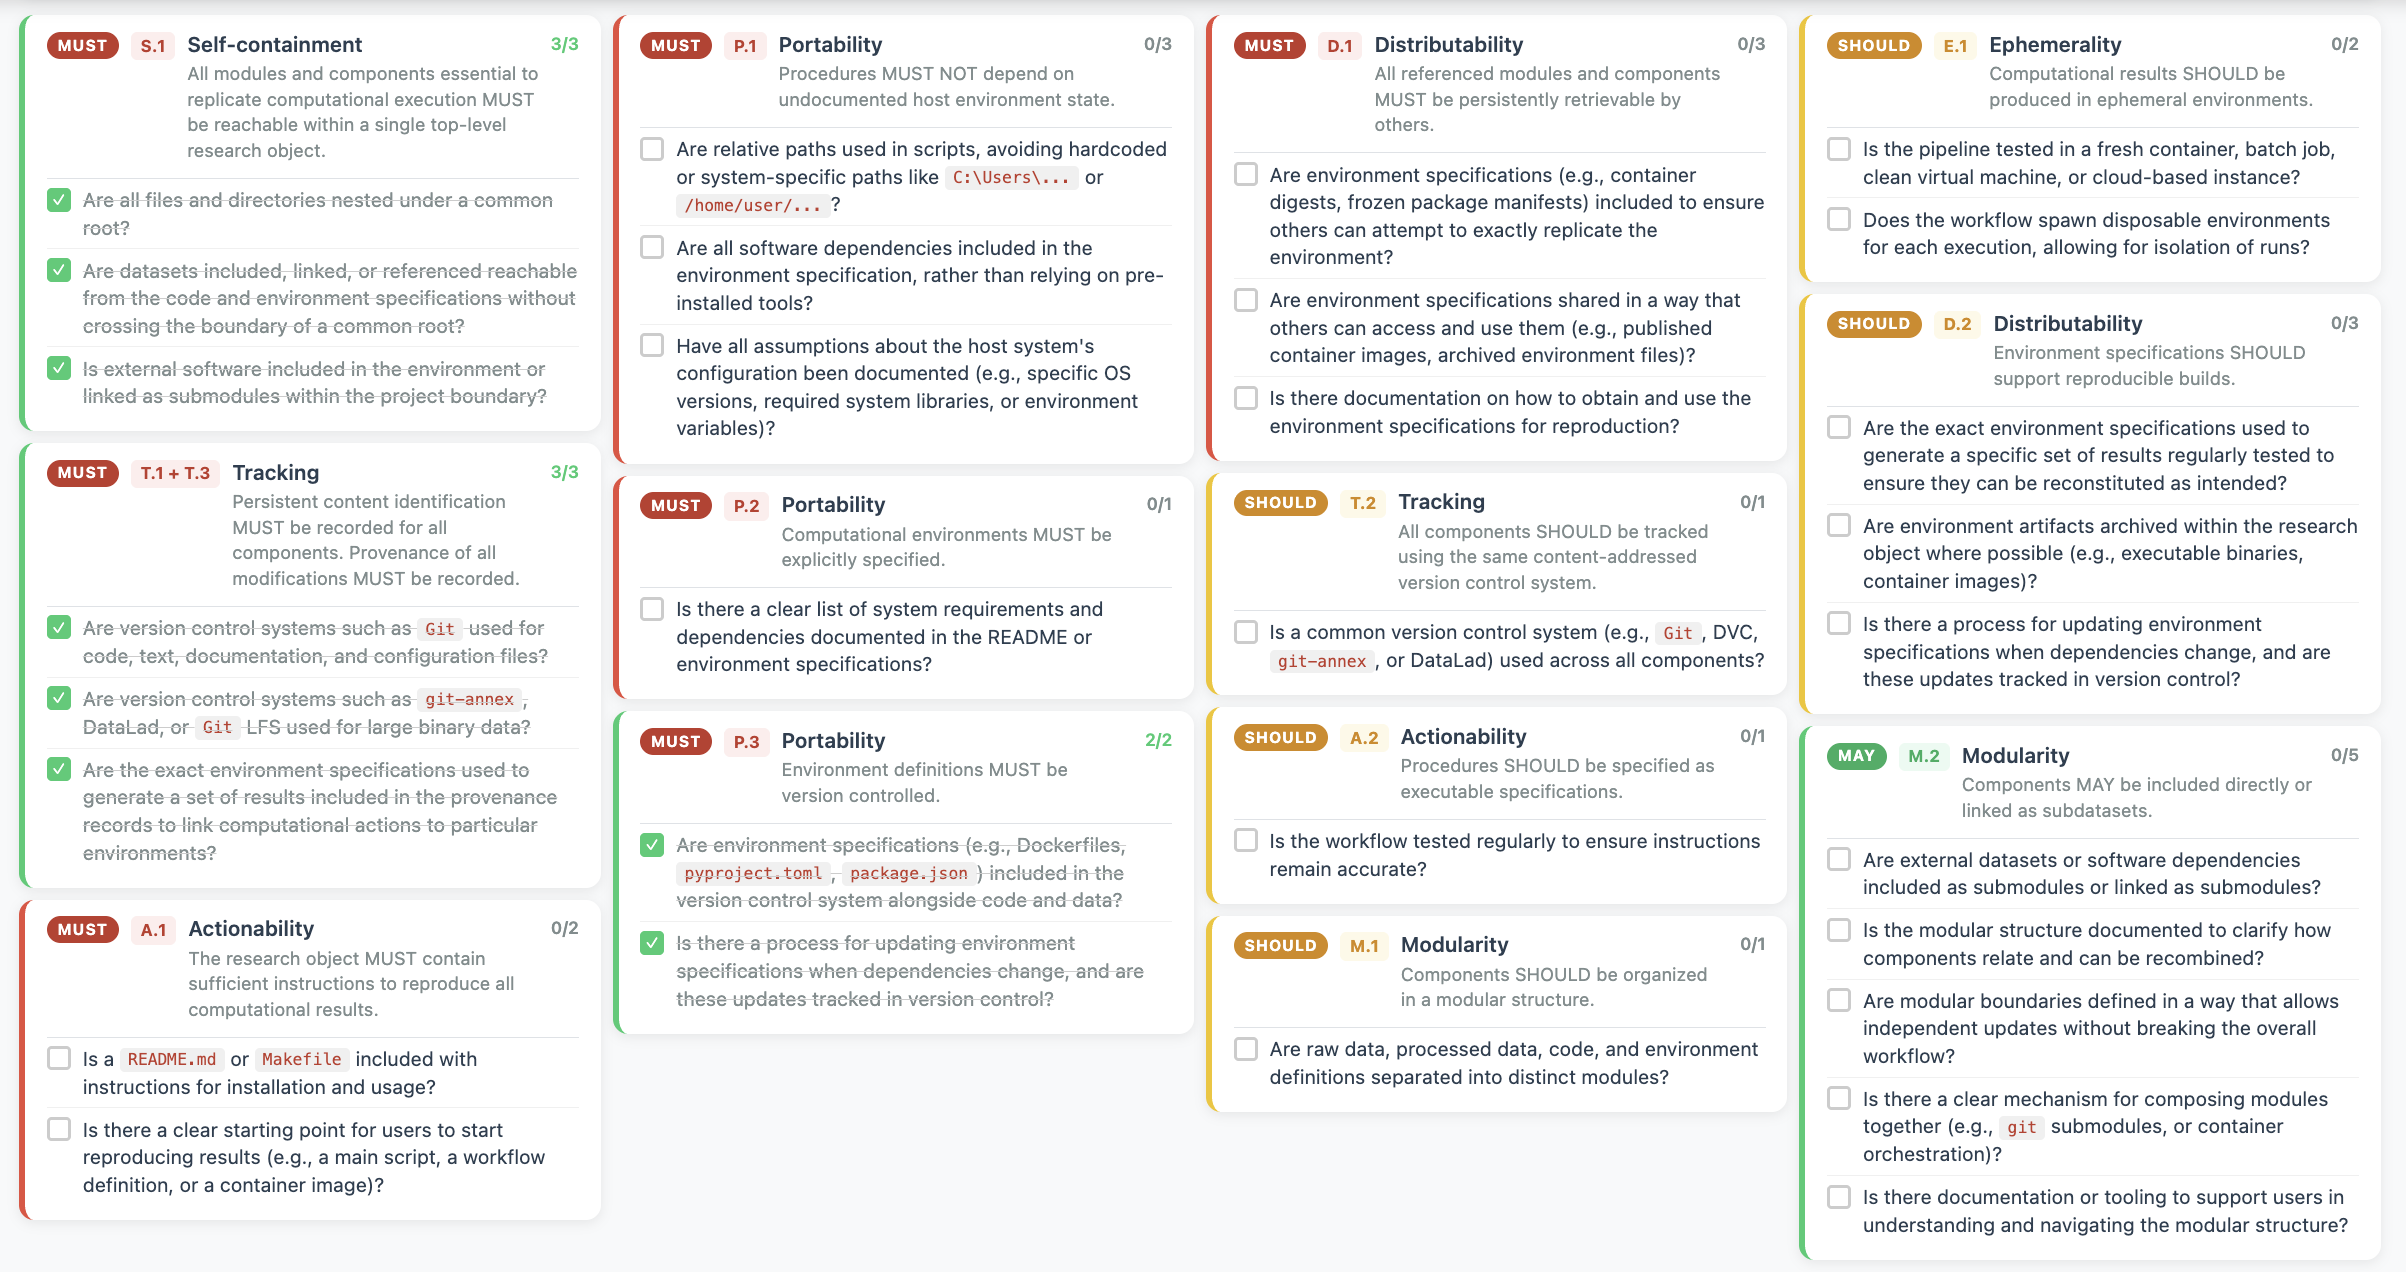
\includegraphics[width=\textwidth]{figures/checklist-figure.png}  % TODO: vectorize
\caption{Screenshot of the interactive checklist for helping guide a workflow developer through common cases.}
\label{fig:stamped}
\end{figure}





\subsection{Enabling tools}

No single tool addresses all the dimensions of scientific rigor described above, though many tools contribute to one or several properties simultaneously.
For example, container technologies such as Docker or Singularity serve Portability by providing OS-level isolation from explicit environment specifications, enable Ephemerality by disposing per-execution environments, and facilitate Distributability by producing frozen, shareable artifacts.
Similarly, version control systems such as Git underpin both Tracking (content-addressed identification and change history) and Self-containment (gathering all components under a single root).

In practice, self-containing all data might be undesired or prohibitive due to size or other concerns. Extensions such as git-annex, DataLad, DVC, and Git LFS strike the balance between the two principles by tracking metadata that identifies specific data versions and obtainability information instead, e.g., content checksums and URLs of remote servers that act as a source, and providing actionable interfaces to obtain the data when necessary.

This overlap is not incidental — it reflects the interdependence of the STAMPED principles themselves.
Achieving Ephemerality, for instance, inherently exercises Portability and Actionability; a disposable environment must be reconstituted from explicit specifications, encouraging end-to-end automation.
Likewise, Distributability builds on Self-containment and Tracking; a research object can only be shared in a consistent, retrievable state if its boundary is well-defined and all components are precisely identified.
The tools that enhance multiple properties of a research object do so precisely because they operationalize these connections.

Table~\ref{tab:stamped-tools} maps some commonly used tools and technologies to each STAMPED principle.
A comprehensive up-to-date review of existing tools is out of scope for this formalization paper and would quickly become outdated.
To fill that niche, we initiated a satellite project with a website to describe tools and examples, and characterize them in terms of STAMPED and FAIR principles [cite https://examples.stamped-principles.org].

STAMPED principles are tool-agnostic.
A well-chosen tool can improve several properties at once, and a thoughtfully assembled toolchain can cover all of them.
Researchers should select tools based on their domain, infrastructure, and team familiarity, recognizing that the tools listed here are illustrative rather than prescriptive.
What matters is that the underlying property is satisfied, regardless of which tool achieves it.
Where multiple tools enhance the same STAMPED property of an object, the choice between them often involves trade-offs between flexibility and simplicity.

A representative example is the choice between git-annex and Git LFS for large-file tracking.
Both appear under Self-containment and Tracking in Table~\ref{tab:stamped-tools}, but they occupy different points on a complexity-flexibility spectrum.
git-annex supports many remote types (e.g. other git repositories over SSH or HTTP, or simple cloud data stores such as S3, local drives, offline USB archives), making it well-suited to multi-institutional collaboration, long-term archival where data sovereignty or offline access is required, as well as local content tracking.
Git LFS offers a simpler alternative: it is transparent to users, natively supported by GitHub and GitLab, and broadly adopted.
But it is centralized (requiring an LFS server), lacks offline capability, and provides less flexible remote configurations.
Lightweight STAMPED implementations using Git LFS are entirely feasible for easier onboarding, trading federation flexibility for reduced operational overhead.
The same pattern of flexibility versus simplicity recurs across other tool choices in Table~\ref{tab:stamped-tools}: container-based versus package-based environment management, workflow engines versus shell scripts, and distributed archives versus centralized platforms.

\begin{table}[htbp]
\centering
\caption{Sample tools to improve scientific practice for each STAMPED principle.}
\label{tab:stamped-tools}
\begin{tabular}{|l|p{0.3\textwidth}|p{0.35\textwidth}|}
\hline
\textbf{Principle} & \textbf{Tools / Technologies} & \textbf{Role} \\
\hline
\textbf{S — Self-containment} &
Git submodules, DataLad, git-annex, DVC, Git LFS &
Gather all components (code, data, environments) under a single root via direct inclusion or explicit references (e.g., subdatasets, registered URLs) \\
\hline
\textbf{T — Tracking} &
Git, git-annex, DataLad, DVC, Docker and other containers, Kedro, Git LFS, OSF.io, Zenodo and other data archives providing DOIs &
Version control for code and data; content-addressed identification; provenance recording (e.g., \texttt{datalad run} for programmatic provenance capture); persistent identifiers for content (DOIs) \\
\hline
\textbf{A — Actionability} &
Make, Snakemake, Nextflow, CWL, \texttt{datalad run}, \texttt{git annex addcomputed} &
Define executable specifications for workflows; provide clear entry points for reproducing results \\
\hline
\textbf{M — Modularity} &
Git submodules, DataLad subdatasets, Kedro &
Organize components into independently versioned, composable modules; provide project templates with logical directory separation \\
\hline
\textbf{P — Portability} &
Docker, Singularity, Nix, conda, pip (\texttt{pyproject.toml}, \texttt{requirements.txt}), npm &
Explicitly specify and isolate computational environments; container-based (OS-level isolation) or package-based (declarative, reproducible builds) \\
\hline
\textbf{E — Ephemerality} &
Docker, Singularity, Docker Compose, Slurm, cloud deployments (e.g., AWS, GCP, Azure, GitHub Actions) &
Spawn disposable, temporary environments per execution; validate that specifications are complete by reconstituting from scratch \\
\hline
\textbf{D — Distributability} &
Zenodo, PyPI, conda-forge, DockerHub/GHCR, RO-Crate, \texttt{npm ci}, \texttt{pip freeze}, executable compilers &
Archive and persistently host frozen, versioned research objects and their components; enable retrieval by others in the intended state \\
\hline
\end{tabular}
\end{table}



\subsection{Examples and Case Studies}

\subsubsection{Pedagogical examples}

To complement the formal definitions above, the satellite examples project (\url{https://examples.stamped-principles.org}) walks the reader through the STAMPED properties using small, concrete worked examples.
The pages tagged ``STAMPED-intro'' (\url{https://examples.stamped-principles.org/tags/stamped-intro/}) trace how each property applies to the same simple research object, providing a gentle on-ramp before the real-world adoptions below.

\subsubsection{Real-world adoptions}

Several research projects have already adopted and documented the YODA principles (the predecessor to STAMPED) demonstrating practical utility across domains.

\textbf{BIDS Standard Evolution}: A significant validation of the ``do not look up'' principle occurred within the Brain Imaging Data Structure (BIDS)\cite{gorgolewski_brain_2016} community.
Originally, the BIDS specification nested derived data under \texttt{derivatives/} within the original raw dataset, creating upward dependencies that violated portability.
Following YODA principles, the BIDS community reversed this relationship so that derivative datasets now exist independently and reference raw data as subdatasets, not vice versa.

This architectural shift influenced major neuroimaging tools:
\begin{itemize}
    \item \textbf{fMRIPrep}: Switched default output layout to follow YODA structure
    % TODO: add GitHub issue reference for "yoda" layout proposal
    \item \textbf{OpenNeuroDerivatives}: Entire derivative dataset collection now follows YODA organization, separating processed outputs from raw data dependencies
    \item \textbf{BIDS specification}: Updated to accommodate and recommend YODA-compliant layouts for derivative datasets
\end{itemize}

\textbf{Workflow Platforms}: Infrastructure projects implementing YODA at scale:
\begin{itemize}
    \item \textbf{BABS}\cite{zhao_reproducible_2024}: Platform implementing the ``FAIRly big workflow'' approach, demonstrating YODA principles for large-scale neuroimaging analyses with containerized pipelines and modular dataset composition
    \item \textbf{CRCNS.org}: Neuroscience data sharing platform providing YODA-structured templates and validation tools
\end{itemize}

These adoptions demonstrate that STAMPED principles solve practical organizational challenges across scales, from individual studies to community-wide infrastructure.

\subsection{Convergent evolution of data-driven scientific practices}

The challenges that motivate STAMPED are not unique to any single domain.

Fragmented provenance, irreproducible computations, and ad-hoc project layouts have plagued communities across geophysics, statistics, genomics, neuroimaging, and machine learning for three decades.
Independently, each converged on strikingly similar organizational responses.
What follows is not a comprehensive review but a tracing of that convergence, organized chronologically, to show that the principles STAMPED formalizes reflect durable responses to recurring challenges.

The earliest calls for reproducibility-as-organization appeared in the 1990s.
Claerbout and Karrenbach\cite{claerbout_electronic_1992} demonstrated that coupling electronic documents with Makefiles could make geophysical analyses self-contained, tracked, and re-executable---anticipating Self-containment~(S), Tracking~(T), and Actionability~(A).
Buckheit and Donoho\cite{bickel_wavelab_1995} extended this idea with WaveLab, a compendium packaging code, data, and figures so that ``an article \ldots{} is not the scholarship itself, \ldots{} the actual scholarship is the complete software development environment and the complete set of instructions which generated the figures''---touching Self-containment~(S), Actionability~(A), Portability~(P), and Distributability~(D).
Gentleman and Temple~Lang\cite{gentleman_statistical_2007} formalized the research compendium concept, emphasizing modular packaging for reuse and redistribution---Self-containment~(S), Modularity~(M), Actionability~(A), and Distributability~(D).
Noble\cite{noble_quick_2009} provided the first widely adopted project-organization guide for computational biology, offering concrete directory-structure conventions that addressed Self-containment~(S) and Modularity~(M).

A wave of normative frameworks followed in the 2010s.
Stodden\cite{stodden_scientific_2010} articulated legal and social dimensions of sharing computational research, raising concerns central to Distributability~(D) and Tracking~(T).
Sandve et~al.\cite{sandve_ten_2013} distilled ten rules for reproducible computation (track versions, record workflows, archive environments)---spanning Tracking~(T), Actionability~(A), and Self-containment~(S).
The FAIR principles\cite{wilkinson_fair_2016} established findability, accessibility, interoperability, and reusability as community norms for digital objects, later extended to research software by FAIR4RS\cite{barker_introducing_2022} and to workflows by the Workflow Community Initiative\cite{wilkinson_applying_2025}.
Wilson et~al.\cite{wilson_good_2017} codified ``Good Enough Practices'' that operationalized many of these ideals for working scientists---Actionability~(A), Tracking~(T), and Self-containment~(S).
The YODA principles\cite{hanke_yoda_2018} combined these insights into organizational practices for research data management.
De~Smedt et~al.\cite{de_smedt_fair_2020} articulated the notion of FAIR Digital Objects as ``actionable knowledge units,'' foregrounding Actionability~(A) as a first-class concern complementary to FAIR.
Building on YODA and this emphasis on actionability, the VAMP formulation\cite{hanke_what_2023} (Versioned, Actionable, Modular, Portable) made Actionability~(A), Portability~(P), and Modularity~(M) explicit organizational requirements, and introduced Ephemerality~(E) as validation for Portability~(P)---directly prefiguring STAMPED.
Notably, the WCI-FW framework\cite{wilkinson_applying_2025} extended FAIR to computational workflows but explicitly declined to define new principles, leaving the operational gap  that STAMPED fills (how a research object should be structured and managed).

Independent of these normative efforts, a parallel ``Git for data'' convergence occurred in tooling.
git-annex (2010), Git~LFS (2015), DVC (2017), Pachyderm (2014), and Icechunk (2024) all independently arrived at content-addressed identification of large files, logical separation of metadata from bulk storage, and derivation records linking inputs to outputs.
These systems vary widely in architecture, ranging from cloud-native to local-first and from centralized to distributed.
Despite these differences, each converged on the same core insight, that version-control semantics proven for code could and should extend to data.
This convergence is evidence not of influence but of shared need, and maps most directly onto Tracking~(T).

A complementary convergence emerged in platforms and metadata standards.
Though not an exhaustive list: Galaxy\cite{afgan_galaxy_2018} (first released 2005), Code~Ocean (2017), and brainlife.io\cite{hayashi_brainlifeio_2024} each provided turnkey reproducibility services, each implementing separation of code, data, and environment as a first-class abstraction---reflecting Self-containment~(S), Actionability~(A), and Portability~(P).
On the standards side, the W3C~PROV data model (2013), Frictionless Data (2007), RO-Crate\cite{peroni_packaging_2022}, and BioComputeObject (IEEE~2791-2020) each addressed interoperable packaging and provenance recording.
The facts that FAIR required elaboration to accommodate software\cite{barker_introducing_2022} and workflows\cite{goble_fair_2020,wilkinson_applying_2025}, and that independent standards converged on provenance and packaging, confirms that these dimensions are recurrently demanded by research practice.

Framework tooling and domain standards reveal the same pattern at the project-layout level.
Cookiecutter Data Science (2016), BIDS\cite{gorgolewski_brain_2016} (2016), Kedro (2019), nipoppy (2023), and others, all imposed opinionated directory structures and modular separation (independently motivated by the costs of ad-hoc layouts)---reflecting Modularity~(M) and Self-containment~(S).
Each framework constrains where code and documentation reside, how raw data inputs and derived outputs are handled, which makes such projects navigable by \emph{convention}.

Viewed together, these independent lines of development map onto every STAMPED principle.
Self-containment~(S) appears wherever projects bundle their dependencies into a single rooted structure; 
Tracking~(T) wherever content-addressed storage or version control records the history of changes or acquisition of every component;
Actionability~(A) wherever Makefiles, workflow managers, or platform APIs make re-execution or acquisition a single command;
Modularity~(M) wherever directory conventions or subproject composition separate concerns;
Portability~(P) wherever good coding practice, containers or environment specifications decouple a research object from a particular machine;
Ephemerality~(E) wherever composition brings together computation on data which is treated as disposable and regenerable;
and Distributability~(D) wherever licensing, packaging standards, or data logistic mechanisms enable sharing.

The formalization presented here provides a shared vocabulary for what these practices have in common, enabling researchers to evaluate and incrementally improve their workflows regardless of the specific tools they employ.
Figure~\ref{fig:convergent-evolution} summarizes these parallel timelines and their mapping to STAMPED principles.

\begin{figure}[htbp]
\centering
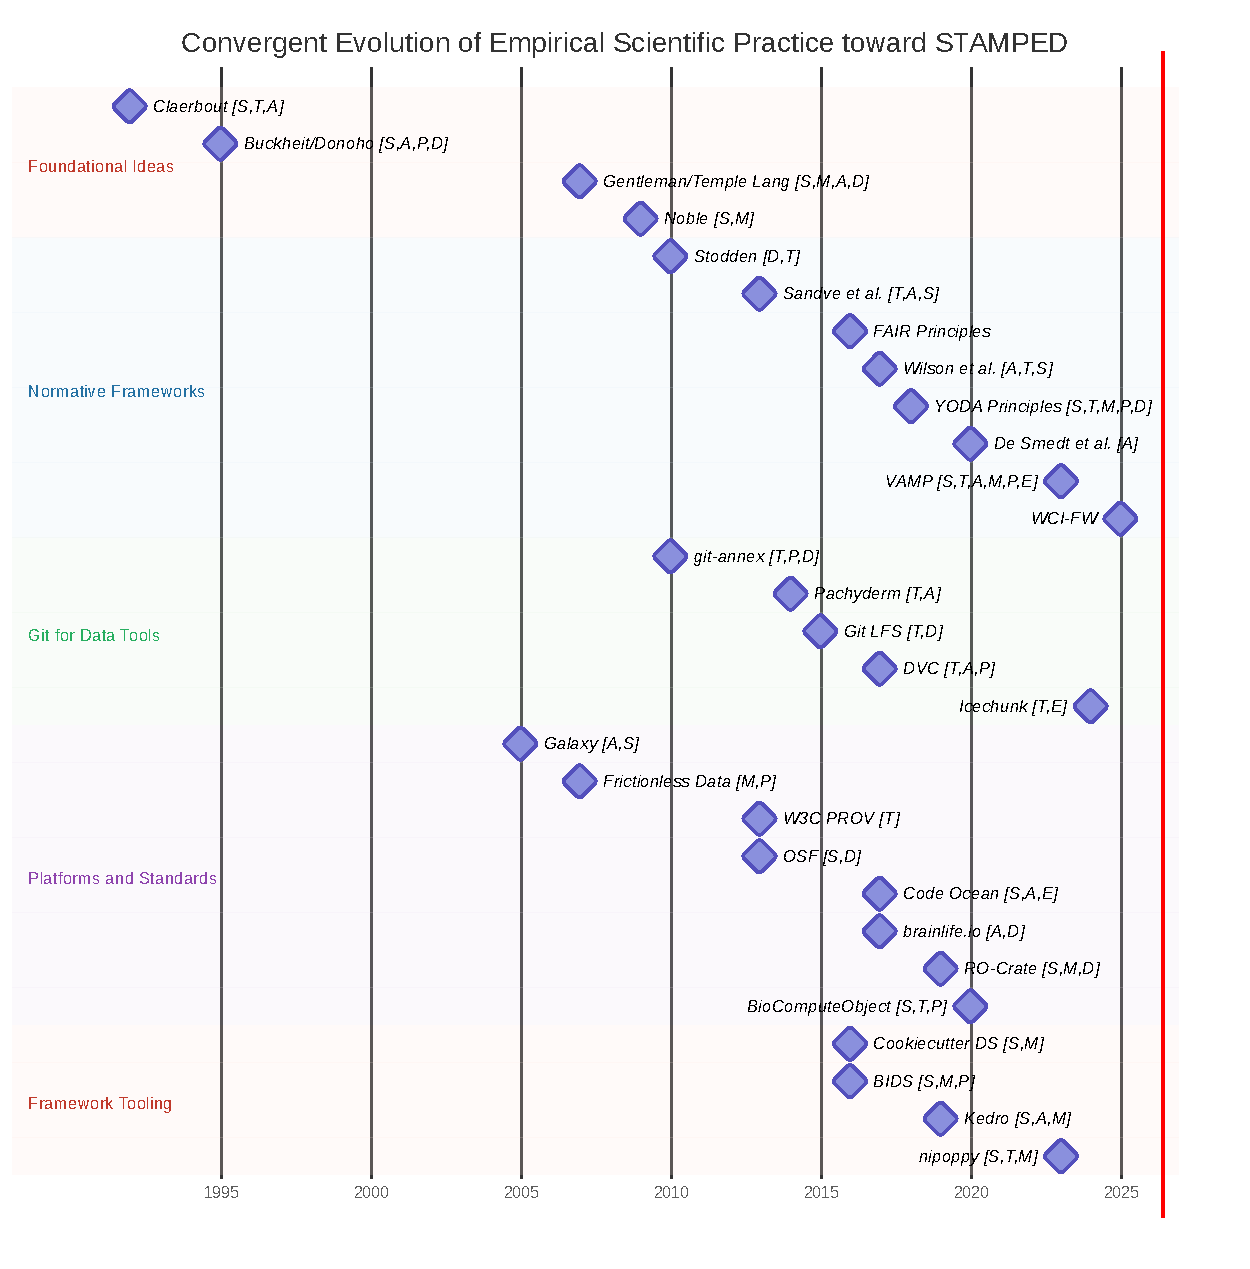
\includegraphics[width=\textwidth]{figures/convergent-evolution-gantt.pdf}
\caption{Convergent evolution of empirical scientific practice toward STAMPED.
Five independent lines of development are shown on a shared timeline from 1992 to 2025.
These comprise foundational ideas, normative frameworks, data version-control tools, platforms and metadata standards, and framework tooling.
Each milestone is annotated with the STAMPED principles it anticipates.
Despite independent origins, all five tracks converged on the same organizational patterns that STAMPED formalizes.
The milestones shown are illustrative rather than exhaustive; many other influential projects and communities contributed to this convergence but are omitted here for brevity.}
\label{fig:convergent-evolution}
\end{figure}



\subsection{Future Directions}

STAMPED principles provide a vocabulary rather than a closed specification, which is rooted in practices that continue to evolve with tooling, policy, and scientific convention.
The directions below identify open fronts where the framework's vocabulary will need to stretch, and where complementary work by adjacent communities will shape how STAMPED assists researchers in the coming decade.
We begin with directions that apply broadly across computational science, including generalizing Ephemerality to workflow specifications, aligning provenance standards, building adoption incentives, and seeding training pipelines.
The remainder of the section then addresses the more specific and fast-moving challenges introduced by AI, where several STAMPED principles need explicit extensions and where the stakes for transparent, reproducible research are most immediate.

\subsubsection{Specification-centric research objects as the reproducibility ideal}

Ephemerality (E), as formulated here, treats the compute environment as disposable while the code and data it runs on remain durable.
A complementary view is emerging in which workflow implementations themselves become regenerable from a durable specification.
Declarative workflow languages such as CWL\cite{crusoe_methods_2022}, Snakemake\cite{molder_sustainable_2021}, and Nextflow\cite{di_tommaso_nextflow_2017}, together with fully-declarative environment managers such as Nix and Guix, already operate this way.
The specification accumulates the domain knowledge, including inputs, constraints, expected outputs, and validation criteria, while any given implementation can be rebuilt or replaced without loss.
Under this view, STAMPED principles apply to the specification first and the generated implementation second.
The specification is what must be Self-contained, Tracked, Actionable, and Distributable, while the running code is ephemeral in the same sense as a container.
The connection to pre-registration is direct and generalizes Ephemerality even further\cite{nosek_preregistration_2018}.
A well-formulated study specification is a commitment that survives any particular implementation, and what is ephemeral expands from the compute environment to the full ``scientific middleware'' (data acquisition, harmonization, preprocessing, analytics), with each stage reduced to a specification from which implementations can be derived.
That is where concentration on formalization and standardization of overall study specifications becomes the target to apply STAMPED principles, so that the middleware steps could also be automatically carried out in an ephemeral fashion and potentially while exploring various possible implementations.
The cost of under-specified middleware is already visible in practice; the NARPS study showed that 70 independent teams analyzing the same fMRI dataset with nominally similar hypotheses produced substantially divergent results\cite{botvinik-nezer_variability_2020}, precisely because the study specification left most of the middleware up to each team.
% Here could potentially point to the opposite -- Ben's agentic AI being capable of support/demonstrating core "behavioral neuroscience" paradigms. TODO: citation? mention in AI subsection?


\subsubsection{Provenance standards convergence}

As FAIR leaves specific protocols and standards open, STAMPED likewise does not prescribe a serialization for provenance records, and in practice researchers rely on whatever their tooling emits.
Convergence among existing approaches would let STAMPED research objects carry portable provenance across toolchains without lock-in.
Relevant efforts include cross-domain standards such as W3C PROV\cite{w3c_provenance_working_group_prov-overview_2013} and RO-Crate\cite{peroni_packaging_2022}, tool-level records such as DataLad's\cite{halchenko_datalad_2021} \texttt{datalad run} provenance, and domain-specific specifications such as BIDS-Prov (BEP028)\cite{bids_community_bep028_2025}.
This is less a change to STAMPED itself than a call on these communities: Tracking (T) becomes substantially more useful when provenance records follow shared standards and can be exported, compared, and re-interpreted by tools other than the one that generated them.


\subsubsection{Adoption incentives and tool certification}

STAMPED compliance today is self-assessed against the checklist fulfilling a simple LinkML model\cite{stamped-checklist-schema:v0.1.0}, which then presented in this paper, and exposed to users in a convenient Web UI at \url{https://checklist.stamped-principles.org}.
That Web UI provides self-contained stateful permalinks to render any particular state of the filled out checklist, so they could be shared easily.
Broader adoption will depend on promotion and external incentives, including funder mandates (e.g.,\ NIH Data Management and Sharing policies), journal reproducibility badges\cite{center_for_open_science_open_2023}, and venue-level review checklists that converge toward automated scoring. 
Such a trajectory would parallel that of FAIR, which has moved from principles to machine-assessable indicators with tools such as F-UJI\cite{devaraju_automated_2021}.
No automated tool yet available as of now certifies STAMPED compliance.
A community-maintained benchmark suite, seeded by the satellite examples project associated with this paper (\url{https://examples.stamped-principles.org}), is a natural precursor.


\subsubsection{Teaching and onboarding}

Uptake through formal training is slow but compounding: as the ``train the trainer'' model used by the ReproNim program has demonstrated, students and early-career researchers who encounter these practices during training become some of the most effective propagators of the vocabulary, even if that propagation takes years to surface.
Existing resources already teach most of what STAMPED asks for, without using the term.
These include EduWrench\cite{casanova_eduwrench_2023}, the Reproducible Research MOOC which teaches \texttt{git-annex} and related tools\cite{legrand_reproducible_2022}, and RDMkit data analysis best practices\cite{elixir_rdmkit_community_data_2024}.
Curricular integration with open-science and neuroimaging training programs such as Brainhack would close the gap between practitioners who apply these practices by habit and those who can name what they are doing and evaluate it against a shared checklist.
YODA principles have already entered the curricula of several such programs, and we expect their references to migrate toward the more formally articulated STAMPED vocabulary.
Continued community outreach, including a recent introduction to STAMPED\cite{baker_guidelines_2026} delivered to the BRAIN BBQS program, supports that transition.


\subsubsection{Research in an AI Era}

AI agents are now generating analysis code, selecting methods, and in some systems running entire research cycles end-to-end\cite{boiko_autonomous_2023, lu_ai_2024, mitchener_kosmos_2025}.
Without explicit structure, this automation can produce results whose provenance and reasoning are irrecoverable\cite{messeri_artificial_2024}.
The STAMPED principles already carry most of what is needed.
Self-contained workspaces alone give agents a well-defined boundary; Tracked histories make agent contributions auditable and contribute to their ``memory''; Actionable documentation serves humans and machines alike.
As with any new methodology or instrumentation entering science, several of these principles need AI-era extensions.
Because the agentic-AI ecosystem is evolving rapidly, the directions below are indicative rather than exhaustive.

\paragraph{Self-contained models.}
Machine learning models are becoming standard components of research workflows, yet they are often fetched at runtime from external repositories with no guarantee of long-term availability or version stability.
Users frequently interact with models through platforms without knowing which model version produced their results.
Even where models are nominally versioned the degree of control varies widely, with Hugging Face providing commit-level pinning while commercial APIs may silently update the model behind a fixed endpoint.
Self-containment (S) extends naturally to this case: models are tracked components of the research object, just as data and code are today.
Practical mechanisms exist for open models, such as pinned revisions on Hugging Face or, for durable self-containment, archival copies managed via \texttt{git-annex}.
Tracking what training data and procedures produced a given model remains an open problem that intersects copyright, benchmarking, and provenance, and is mostly beyond what STAMPED can prescribe.
Community artifacts such as Model Cards\cite{mitchell_model_2019} and Datasheets for Datasets\cite{gebru_datasheets_2021} nonetheless point toward the shape of an answer.

\paragraph{Provenance for AI-driven changes.}
When an AI agent modifies code, generates analysis scripts, or makes architectural decisions, those actions become part of the research record.
Tracking (T) naturally extends to cover agent actions by wrapping an agent invocation in a provenance-capturing command such as \texttt{datalad run} records the model, prompt, and resulting changes alongside the output.
Some of this provenance is already captured organically through git commits authored by agents, session transcripts, and co-authorship metadata.
Emerging tools such as Entire CLI\cite{entire_entire_2026} go further, automating capture of the entire AI session alongside the commit.
A practical tension follows wherein agent sessions can produce enormous transcripts, and including them wholesale may dilute the value of more targeted provenance records, so what to capture and at what granularity remain open questions.
Bitwise reproducibility is not the target and rarely is the goal even for human-driven steps.
Instead, what the record must preserve is the hypothesis, the method specification, and enough of the decision trail to support introspection.
Self-contained models (above) strengthen this chain---when the model itself is tracked, the provenance record is more complete.

\paragraph{Machine-actionable instructions.}
Actionability (A) was defined with human operators in mind, including entry-point commands documented in READMEs, frequently incomplete or out of sync with the underlying workflow.
AI agents are a second consumer of the same prose, one that can parse, follow, and correct instructions on the fly, and plain Markdown has effectively become the interface language: \texttt{CLAUDE.md} files, README-driven agent workflows, and spec-kit\cite{github_spec_2025} collections now function as machine-actionable interfaces, making Self-contained and Tracked research objects more Actionable.
Where prose instructions fail, the failure is legible (an audit mechanism that did not exist before) even if agent-driven execution remains less reliable than deterministic tooling.

\paragraph{AI-accelerated specification-to-implementation.}
Specification-centric research objects (above) depend on the cost of regenerating an implementation from a specification being low enough to be routine.
AI coding assistants and specification-driven toolkits such as spec-kit move this cost toward zero, making the spec-centric view practical rather than aspirational.
This holds provided the preceding extensions for models, provenance, and machine-actionable instructions are in place.
This closes a loop with the end-to-end ``AI scientist'' systems that opened this section\cite{boiko_autonomous_2023, lu_ai_2024, mitchener_kosmos_2025}.
As soon as an agentic pipeline takes a study specification and returns data, code, figures, and a draft manuscript, the specification and every downstream artifact must together satisfy STAMPED, not only to keep such pipelines efficient to re-run at lower cost but to make their outputs introspectable.
Tracked and self-contained research objects let a researcher inspect which model, prompt, and decision led to a particular result, implement ``hand over'' between humans and agents alike and let subsequent actor re-enter a prior state and continue from it without rediscovering context.
At the end, human scientists authoring and iterating over the specification of a STAMPED research object would see how their edits propagate through the generated implementation.
Without the STAMPED principles, the acceleration might be real but the accountability would be lost.
Instead, spec-driven agentic research becomes a collaborative, transparent artifact between scientists and the AI systems that support them.


\section{Data Availability}

% TODO

\section{Code Availability}

% TODO


\bibliographystyle{unsrtnat}
\bibliography{references}

\section{Author Contributions}

\section{Competing Interests}
The authors declare no competing interests.

\section{Acknowledgments}

This manuscript and companion materials in the \href{STAMPED Principles GitHub organization}{https://github.com/stamped-principles/} were prepared with the assistance of agentic AI coding tools and large language models (primarily Claude Opus).
All final text, figures, and specifications were edited and/or confirmed by the human authors, who are responsible for the content.
Where AI tools notably contributed to a change, we have strived to annotate the corresponding commits with a \texttt{Co-Authored-By} trailer, or analogous comments, to identify the tool and potentially the model version, so that the provenance of individual contributions is inspectable in the public git history of the \texttt{stamped-*} repositories.

\section{Funding}
This work was supported by the National Institutes of Health:
ReproNim --- Center for Reproducible Neuroimaging Computation (NIBIB P41~EB019936),
OpenNeuro --- An Open Archive for Analysis and Sharing of BRAIN Initiative Data (NIMH R24~MH117179),
DANDI --- Distributed Archives for Neurophysiology Data Integration (NIMH R24~MH117295),
and EMBER --- Ecosystem for Multi-modal Brain-behavior Experimentation and Research (NIMH R24~MH136632).

\end{document}

% LocalWords:  agentic
